% ###################    CONFIGURACIÓN ################### 

% Configuración de estilos generales de la página
\documentclass[12pt,
               % twocolumn
              ]{article}
              
\usepackage[paperheight=297mm,
			paperwidth=210mm,
			tmargin=28mm, 
			headheight=0mm, 
			headsep=15mm,
			textheight=240mm,
			footskip=7mm,
			textwidth=159.2mm,
			bindingoffset=10mm,
			twoside
			]{geometry} 
% -------------------------------------------------------   


% Configuración de párrafos
% -------------------------------------------------------         
\setlength{\parindent}{0em} % Tabulación de un párrafo nuevo
\setlength{\parskip}{1em}   % Distancia en blanco entre un párrafo y otro.
\setlength{\columnsep}{1em} % Margen izquierdo de columnas
\renewcommand{\baselinestretch}{1.5} % Interlineado. Espacio entre dos renglones.
% ------------------------------------------------------- 


% Paquetes de idioma
\usepackage[utf8]{inputenc}
\usepackage[spanish,english,es-tabla]{babel} % English para el abstract
% ------------------------------------------------------- 

% Paquetes generales
\usepackage{enumitem} % Para configurar enumeraciones
\usepackage[usenames,dvipsnames]{xcolor,colortbl}    % Para colores en el texto

\usepackage{float} % para controlar la situación de los entornos flotantes

\usepackage{graphicx} % figuras

\usepackage{subcaption} % Para subfiguras

\usepackage{wrapfig} % Para poner imagen al lado del texto

\usepackage{fancyhdr} % Para los encabezados y pie de página

% Definimos un nuevo color
\definecolor{webred}{rgb}{0.5, 0, 0}   % less intense red

% Colores para la tabla

\definecolor{azulOscuro}{RGB}{102,101,205}
\definecolor{azulClaro}{RGB}{235,244,255}
\definecolor{amarilloSuave}{RGB}{255,252,158}
\definecolor{verdeSuave}{RGB}{154,255,153}
\definecolor{rojoSuave}{RGB}{253,104,100}

\usepackage[bookmarks=true,
			bookmarksnumbered=false, % true means bookmarks in 
									 % left window are numbered                         
			bookmarksopen=false,     % true means only level 1
									 % are displayed.
			colorlinks=true,
			linkcolor=webred,
			citecolor=webred,
			%linkcolor=OliveGreen,
			urlcolor=cyan]{hyperref} % Para hiperenlaces

% Definimos una nueva orden para pintar una línea cuando escribamos \HRule
\newcommand{\HRule}{\rule{\linewidth}{1mm}}

% Se define el estilo de cabecera y pie de página

\fancypagestyle{miEstilo}{
   \lhead{\leftmark}
   \rhead{Página \thepage}
   \lfoot{}
   \cfoot{}
   \rfoot{}
}


% Definimos el título y autor de la página

\title
{	
	\vspace{-3cm}
	\begin{figure}[!h]
				\centering
				
\includegraphics[scale=0.35]{images/logo_ugr}
	\end{figure}
	\pagestyle{empty}
	\HRule 
	\begin{figure}[!h]
				\centering
				
\includegraphics[scale=0.5]{images/portada}
	\end{figure}
	\begin{center}
		\Huge 
		\texttt{Análisis comparativo de bases de datos relacionales y no relacionales}\\[6mm]
	\end{center}
	\HRule 
}

\author{\large Jonathan Martín Valera}


% ###################   FIN CONFIGURACIÓN ################### 

% ###################	INICIO DEL DOCUMENTO ###################

\begin{document}

\selectlanguage{spanish}

\maketitle
\thispagestyle{empty} % Se quita el número de página en la portada

\newpage

\thispagestyle{empty}

\vspace*{\fill} % Para alinear el contenido de la paǵina verticalmente.

\begin{abstract}

\noindent Los sistemas de gestión de bases de datos relacionales han sido la tecnología predominante para almacenar datos estructurados en aplicaciones web y de negocio. Estos son ampliamente conocidos como bases de datos \texttt{SQL}. Sin embargo, en los últimos años, las bases de datos no relacionales han aumentado drásticamente en popularidad. Estas bases de datos se conocen comúnmente como bases de datos \texttt{NoSQL}, las cuáles son claramente diferentes a las bases de datos \texttt{SQL}.

\vspace{0.3cm}

\noindent El objetivo de este artículo es realizar una breve introducción sobre los fundamentos de las bases de datos, y llevar a cabo un estudio sobre las ventajas e inconvenientes del uso de bases de datos \texttt{SQL} y \texttt{NoSQL}, rendimiento\ldots para saber qué tecnología usar dependiendo del contexto de uso.

\end{abstract}

\selectlanguage{english} 

\begin{abstract}

\noindent Relational database management systems have been the predominant technology for storing structured data in web and business applications. These are widely known as \texttt{SQL} databases. However, in recent years, non-relational databases have dramatically increased in popularity. These databases are commonly known as \texttt{NoSQL} databases, which are clearly different from \texttt{SQL} databases.

\vspace{0.3cm}

\noindent The objective of this article is to make a brief introduction about the basics of the databases, and to carry out a study about the advantages and disadvantages of the use of \texttt{SQL} and \texttt{NoSQL} databases, performance\ldots to know what technology to use depending on the context of use.

\end{abstract}

\vspace*{\fill}

\selectlanguage{spanish}

\newpage

\thispagestyle{empty}

\tableofcontents

\newpage

\thispagestyle{empty}

\listoffigures

\newpage

\pagestyle{miEstilo}

\section{Introducción}

Las bases de datos son el método preferido para el almacenamiento de datos. Desde las grandes aplicaciones multiusuario, hasta los teléfonos
móviles y las agendas electrónicas utilizan tecnología de bases de datos para asegurar la integridad de los datos y facilitar la labor tanto de usuarios como de los
programadores que las desarrollaron \cite{ref1}. 

Además, los datos presentan otra serie de características (uso múltiple, necesidad de acceso eficiente para análisis, necesidad de indexación, etc.), haciendo todas ellas que sea recomendable el uso de bases de datos y tecnologías específicas para su manejo. % Sección 1

\section{Fundamentos de bases de datos}

En esta sección, veremos de forma introductoria esos fundamentos de bases de datos genéricas, aplicables a cualquier ámbito \cite{ref2}.

\subsection*{¿Qué es una base de datos?}

Entendemos como \texttt{Base de Datos} un conjunto de datos estructurado y almacenado de forma sistemática con objeto de facilitar su posterior utilización. Una base de datos puede, por tanto, constituirse con cualquier tipo de datos.

\subsection*{¿Por qué interesa usar una base de datos?}

Las ventajas de utilizar un almacenamiento estructurado se aprecian en diversos puntos, ya que afectan no solo a los datos sino también al propio uso que se hace de estos. Algunas ventajas que afectan directamente a los datos son las siguientes \cite{ref3}:

\begin{itemize}
   \item \textbf{Mayor independencia.} Los datos son independientes de las aplicaciones que los usan, así como de los usuarios.
   
    \item \textbf{Mayor disponibilidad.} Se facilita el acceso a los datos desde contextos, aplicaciones y medios distintos, haciéndolos útiles para un mayor número de usuarios.
    
    \item \textbf{Mayor seguridad (protección de los datos).} Por ejemplo, resulta más fácil replicar una base de datos para mantener una copia de seguridad que hacerlo con un conjunto de ficheros almacenados de forma no estructurada. Además, al estar centralizado el acceso a los datos, existe una verdadera sincronización de todo el trabajo que se haya podido hacer sobre estos (modificaciones), con lo que esa copia de seguridad servirá a todos los usuarios.
    
    \item \textbf{Menor redundancia.} Un mismo dato no se encuentra almacenado en múltiples ficheros o con múltiples esquemas distintos, sino en una única instancia en la base de datos. Esto redunda en menor volumen de datos y mayor rapidez de acceso.
    
    \item \textbf{Mayor eficiencia en la captura, codificación y entrada de datos.} 
\end{itemize}

Esto tiene una consecuencia directa sobre los resultados que se obtienen de la explotación de la base de datos, presentándose al respecto ventajas como, por ejemplo:

\begin{itemize}
 \item \textbf{Mayor coherencia.} La mayor calidad de los datos que se deriva de su mejor gestión deriva en mayor calidad de los resultados.
 
 \item \textbf{Mayor eficiencia.} Facilitando el acceso a los datos y haciendo más sencilla su explotación, la obtención de resultados es más eficiente.
 
 \item \textbf{Mayor valor informativo.} Resulta más sencillo extraer la información que los datos contienen, ya que uno de los cometidos de la base de datos es aumentar el valor de estos como fuente de información. 
\end{itemize}

De forma resumida, puede decirse que la principal bondad de una base de datos es la centralización que supone de todos los datos con los que se trabaja en un contexto determinado, con las consecuencias que ello tiene para una mejor gestión, acceso o estructuración de estos.

\subsection*{Tipos de base de datos}

Existen varios tipos de bases de datos; cada tipo de base de datos tiene su propio modelo de datos (la manera de cómo están estructurados). Entre ellas se incluyen \cite{ref4}:

\subsubsection*{Modelo de base de datos plana}

En un modelo de base de datos plano, hay dos dimensiones (estructura plana) de conjunto de datos. Hay una columna de información y dentro de esta columna, se supone que cada dato tendrá que ver con la columna.

Por ejemplo, un modelo de base de datos plana que sólo incluye códigos postales. Dentro de la base de datos, sólo habrá una columna y cada nueva fila dentro de una columna será un nuevo código postal.

\begin{figure}[!h]
	\centering
	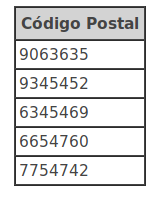
\includegraphics[scale=0.5]{images/tipo_plana}
	\caption{Ejemplo de base de datos plana}
	\label{fig:bd_plana}
\end{figure}

\subsubsection*{Modelo de base de datos jeŕarquica}

El modelo jerárquico de bases de datos se asemeja a la estructura de un árbol, tal como Microsoft Windows organiza las carpetas y archivos. En un modelo jerárquico de bases de datos, cada enlace es anidado con el fin de conservar los datos organizados en un orden particular en un mismo nivel de lista. Por ejemplo, una base de datos jerárquico de ventas, puede incluir las ventas de cada día como un archivo separado. Anidadas dentro de este archivo están todas las ventas (el mismo tipo de datos) para el día.

\begin{figure}[!h]
	\centering
	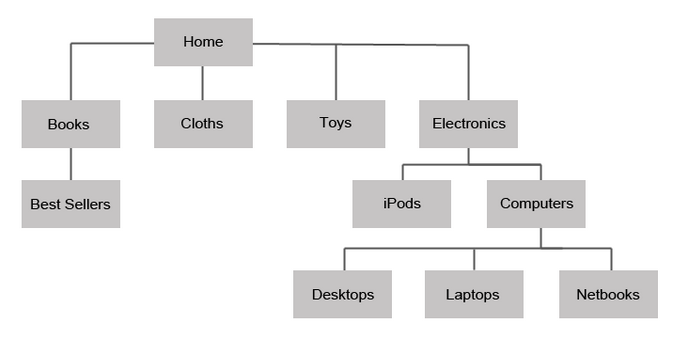
\includegraphics[scale=0.5]{images/tipo_jerarquica}
	\caption{Ejemplo de base de datos jerárquica}
	\label{fig:bd_jerarquica}
\end{figure}

\subsubsection*{Modelo de red}

En un modelo de red, la característica definitoria es que se almacena un registro con un enlace a otros registros - en efecto,una red.

Estas redes (o, a veces, a que se refiere como punteros) puede ser una variedad de diferentes tipos de información como números de nodo de un disco o incluso la dirección. 

\begin{figure}[!h]
	\centering
	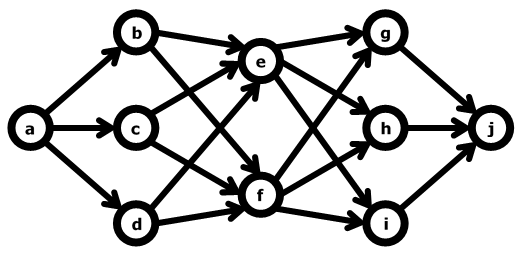
\includegraphics[scale=0.55]{images/tipo_red}
	\caption{Ejemplo de base de datos en red}
	\label{fig:bd_red}
\end{figure}

\subsubsection*{Modelo de bases de datos relacionales}

Las  bases  de  datos  relacionales son un  tipo  de  base  de  datos  que  cumple  con  el  modelo relacional.Consisten en bases de datos separadas en tablas donde cada columna representa un campo y cada fila representa un registro.Cada fila de la tabla tiene una clave única.Las tablas se pueden vincular entre sí con el uso de claves externas o columnas comunes.

\begin{figure}[!h]
	\centering
	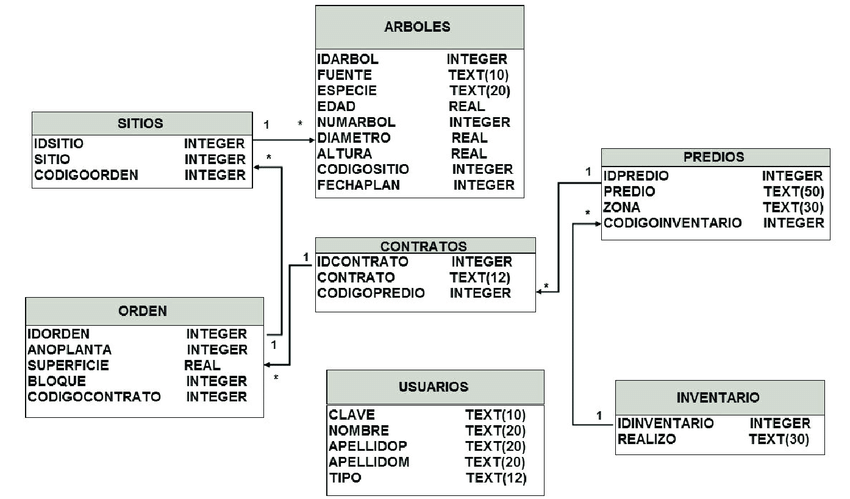
\includegraphics[scale=0.5]{images/tipo_relacional}
	\caption{Ejemplo de base de datos relacional}
	\label{fig:bd_relacional}
\end{figure}

\subsubsection*{Modelo de bases de datos NoSQL}

El término NoSQL que significa Not only SQL(No solamente SQL) fue utilizado por primera vez en 1998 por Carlo Strozzipara nombrar su base de datos de fuente abierta Strozzi NoSQL que no seguía el estándar SQL, pero seguía siendo relacional.

No fue hasta el 2009 cuando Johan Oskarsson, reintrodujo el término NoSQL con la finalidad de etiquetar la aparición de sistemas de almacenamiento de datos distribuidos no relacionales.Una base de datos NoSQL proporciona un mecanismo para el almacenamiento y recuperación de los datos en medios distintos a los utilizados en las bases de datos relacionales.

\begin{figure}[!h]
	\centering
	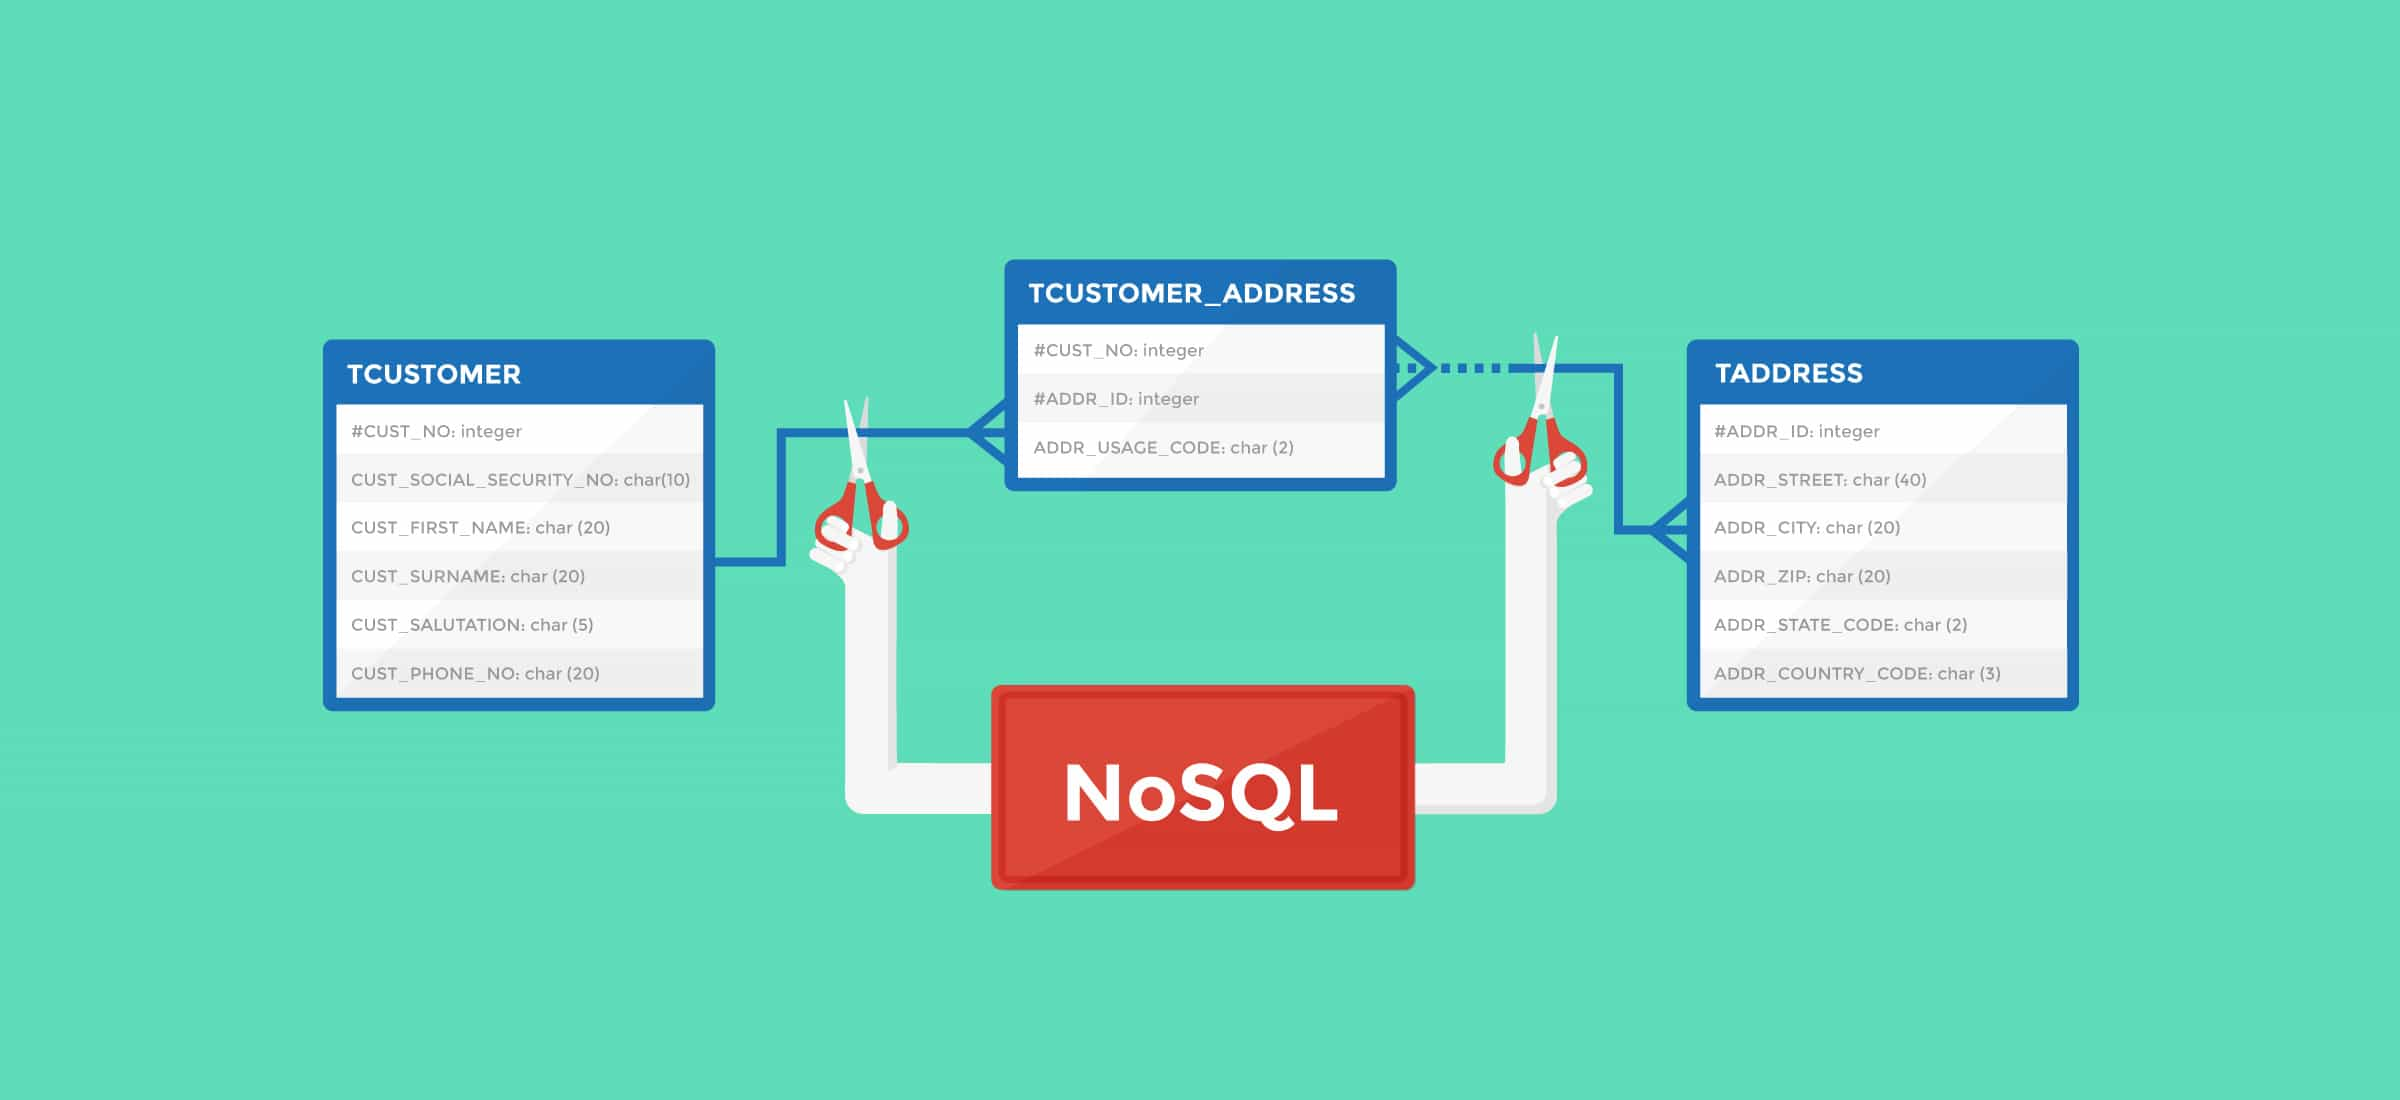
\includegraphics[scale=0.09]{images/tipo_nosql}
	\label{fig:bd_nosql}
\end{figure}

\newpage

\subsection*{Sistema gestor de base de datos}

Un \texttt{sistema gestor de bases de datos} (SGBD) es una aplicación que permite a los usuarios definir, crear y mantener una base de datos, y proporciona acceso controlado a la misma \cite{ref5}.

En general, un SGBD proporciona los siguientes servicios:

\begin{itemize}
	\item Permite la \textbf{definición de la base de datos} mediante el lenguaje de definición de datos (DDL – Data Description Language). Este lenguaje permite especificar la estructura y el tipo de los datos, así como las restricciones sobre los datos. Todo esto se almacenará en la base de datos.
	
	\item Permite la \textbf{inserción, actualización, eliminación y consulta de datos} mediante el lenguaje de manejo o manipulación de datos (DML - Data Manipulation Language). Proporciona un acceso controlado a la base de datos mediante:
	\begin{itemize}
        \item Un sistema de \textbf{seguridad}, de modo que los usuarios no autorizados no puedan acceder a la base de datos, mediante el lenguaje de control de datos (DCL - Data Control Language).
        
        \item Un sistema de \textbf{integridad} que mantiene la integridad y la consistencia de los datos.
        
        \item Un sistema de control de \textbf{concurrencia} que permite el acceso compartido a la base de datos.
        
        \item Un sistema de control de \textbf{recuperación} que restablece la base de datos después de que se produzca un fallo del hardware o del software.
        
        \item Un \textbf{diccionario de datos o catálogo} accesible por el usuario que contiene la descripción de los datos de la base de datos.
	\end{itemize}
\end{itemize}

\newpage % Sección 2

\section{Bases de datos en la actualidad}

Se dice que vivimos actualmente en la era de la información. La oración anterior nos hace pensar un poco en la importancia que tiene la información (o datos) hoy en día, y de la importancia que tiene la preservación de esta información, así como su acceso rápido y eficiente.Todos estos inconvenientes y estas necesidades se pueden resolver con la implementación de bases de datos \cite{ref6}.

Hoy en día podemos hablar sobre dos principales modelos de bases de datos: el modelo \texttt{SQL} y \texttt{NoSQL}.

\begin{figure}[H]
	\centering
	\begin{subfigure}[b]{0.4\textwidth}
		
\includegraphics[width=\textwidth,height=90px]{images/sql}
		\caption{SQL}
		\label{fig:sql}
	\end{subfigure}
	~ 
	\begin{subfigure}[b]{0.4\textwidth}
		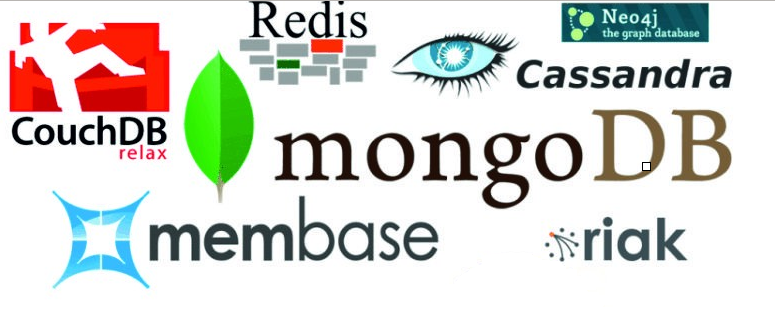
\includegraphics[width=\textwidth,height=90px]{images/nosql}
		\caption{NoSQL}
		\label{fig:nosql}
	\end{subfigure}
	~ 
	\begin{subfigure}[b]{0.5\textwidth}
		
\includegraphics[width=\textwidth,height=90px]{images/sql_o_nosql}
		\caption{¿Cuál elegir?}
		\label{fig:cualelegir}
	\end{subfigure}
\end{figure}

En las siguientes secciones, se detallarán más en profundidad cómo funcionan las bases de datos SQL y NoSQL, y en qué contextos de uso es más apropiado utilizar una u otra.

\newpage % Sección 3

\section{Bases de datos relacionales. SQL}

En el modelo relacional las dos capas de diseño conceptual y lógico, se parecen mucho. Generalmente se implementan mediante \textbf{diagramas de Entidad/Relación} (modelo conceptual) y \textbf{tablas y relaciones} entre éstas (modelo lógico). Este es el modelo utilizado por los sistemas gestores de datos más habituales (SQL Server, Oracle, MySQL...) \cite{ref7}.

El modelo relacional de bases de datos se rige por algunas normas sencillas:

\begin{itemize}

\item Todos los datos se representan en forma de \textbf{tablas} (también llamadas “relaciones”, ver nota anterior). Incluso los resultados de consultar otras tablas. La tabla es además la unidad de almacenamiento principal.

\item Las tablas están compuestas por \textbf{filas} (o registros) y columnas (o campos) que almacenan cada uno de los registros (la información sobre una entidad concreta, considerados una unidad).

\item Las filas y las columnas, en principio, carecen de orden a la hora de ser almacenadas. Aunque en la implementación del diseño físico de cada SGBD esto no suele ser así. Por ejemplo, en SQL Server si añadimos una clave de tipo "Clustered" a una tabla haremos que los datos se ordenen físicamente por el campo correspondiente.

\item El orden de las columnas lo determina cada consulta (que se realizan usando SQL).

\item Cada tabla debe poseer una \textbf{clave primaria}, esto es, un \textbf{identificador único} de cada registro compuesto por una o más columnas

\item Para establecer una relación entre dos tablas es necesario incluir, en forma de columna, en una de ellas la clave primaria de la otra. A esta columna se le llama \textbf{clave externa}. Ambos conceptos de clave son extremadamente importantes en el diseño de bases de datos.

\end{itemize}

Sus principales ventajas son \cite{ref8} :

\begin{itemize}
\item \textbf{Mayor soporte y herramientas} debido a que lleva más tiempo en el mercado.

\item Es una tecnología ampliamente conocida y \textbf{los perfiles que lo conocen son mayoritarios} y más económicos.

\item Las bases de dato relacionales llevan una clase de “cabecera” que permite la \textbf{transaccionalidad entre tablas}. Esto significa que si hay un error durante la petición a cualquier nivel de la operación, se devuelve al punto inicial sin comprometer los datos que fueron utilizados durante el proceso.

\item Los datos deben cumplir con el tipo de dato definido en su estructura.
\end{itemize}

Sus principales inconvenientes son: 

\begin{itemize}
\item No es flexible; todos los objetos ingresados deben tener los mismos campos y estar correctamente validados.

\item El rendimiento y los recursos, mientras más compleja la base de datos y sus relaciones sea debido a la atomicidad, \textbf{necesita más procesamiento}.

\item La escalabilidad es reducida. Una aplicación con SQL \textbf{requiere un aumento de recursos de hardware} que generalmente son bastante costosos para escalar su rendimiento.
\end{itemize}

Algunas tecnologías SQL conocidas son:


\begin{figure}[H]
	\centering
	\begin{subfigure}[b]{0.25\textwidth}
		
\includegraphics[width=\textwidth,height=90px]{images/mysql}
		\caption{MySQL}
		\label{fig:mysql}
	\end{subfigure}
	~ 
	\begin{subfigure}[b]{0.25\textwidth}
		
\includegraphics[width=\textwidth,height=90px]{images/postgres}
		\caption{PostgreSQL}
		\label{fig:postgresql}
	\end{subfigure}
	~ 
	\begin{subfigure}[b]{0.25\textwidth}
		
\includegraphics[width=\textwidth,height=90px]{images/sqlite}
		\caption{SQLite}
		\label{fig:sqlite}
	\end{subfigure}
	
	\begin{subfigure}[b]{0.25\textwidth}
		
\includegraphics[width=\textwidth,height=90px]{images/mariadb}
		\caption{MariaDB}
		\label{fig:mariadb}
	\end{subfigure}
	~ 
	\begin{subfigure}[b]{0.25\textwidth}
		
\includegraphics[width=\textwidth,height=90px]{images/oracle}
		\caption{Oracle}
		\label{fig:oracle}
	\end{subfigure}
	~ 
	\begin{subfigure}[b]{0.25\textwidth}
		
\includegraphics[width=\textwidth,height=90px]{images/sql_server}
		\caption{SQL-Server}
		\label{fig:sqlserver}
	\end{subfigure}
\end{figure}  % Sección 4

\section{Bases de datos no relacionales. NoSQL}

Las bases de datos no relacionales son un \textbf{modelo nuevo} que se ha puesto muy de moda entre desarrolladores Full Stack porque \textbf{no requiere un alto conocimiento académico de bases de datos y su curva de aprendizaje y practicidad lo hacen bastante atractivo para proyectos rápidos}.

NoSQL se compone generalmente de bases de datos, compuestas a su vez por Colecciones que poseen documentos; también hay otras tecnologías NoSQL que poseen columnas y estructuras diferentes

\subsection{Tipos de base de datos no relacionales}

No existe una clasificación universalmente aceptada en las bases de datos NoSQL. A menudo, sin embargo, suelen clasificar las bases de datos según su modelo de datos. Los cinco principales modelos de datos son: bases de datos clave-valor, documentales, orientada a grafos, orientada a columnas y orientada a objetos \cite{ref1}.

\subsubsection{Bases de datos clave-valor}

Las bases de datos clave-valor son bastante simplistas, pero tienen un modelo bastante eficiente y potente. Los datos están formados en dos partes, una cadena que representa la clave y los datos reales a los que se hace referencia como valor, creando así un par \textbf{“clave-valor”}, que es una clave única con la que se identifica cada elemento. El almacén de datos es similar a las tablas de hash donde las claves se utilizan como índices por lo que es más rápido que una base de datos relacional. Los más recientes almacenes de datos prefieren una alta escabilidad sobre la consistencia, por lo tanto, se han omitido operaciones como los joins o funciones de agregado. Algunas bases de datos de este tipo son \textit{Cassandra, Amazon DynamoDB, RIAK}.

\begin{figure}[!h]
	\centering
	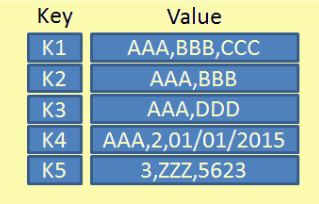
\includegraphics[scale=0.5]{images/nosql_clave-valor}
	\caption{Ejemplo de base de datos clave-valor}
	\label{fig:bd_clave-valor}
\end{figure}

\subsubsection{Bases de datos documentales}

Las bases de datos documentales almacenan sus datos en forma de documentos, generalmente
utilizando como estructura JSON (JavaScript Object Notation) o XML (Extensible Markup
Language). El almacenamiento en documentos ofrece un gran rendimiento y permite la escabilidad
horizontal. Los documentos dentro de una base de datos documental son similares a los registros
dentro de una base de datos relacional pero mucho más flexibles. En las bases de datos relacionales,
un registro dentro de la misma base de datos tendrá los mismos campos para todos los datos y los
campos que no se utilicen se mantendrán vacíos, en las bases de datos documentales cada
documento podrá tener datos similares, así como datos diferentes. Los documentos de la base de
datos utilizan una clave única que representa cada documento. Permite realizar búsquedas por
clave-valor y consultas más complejas sobre el contenido de los datos. Algunas bases de datos de
este tipo son \textit{MongoDB, CouchDB, SimpleDB \ldots}

\begin{figure}[!h]
	\centering
	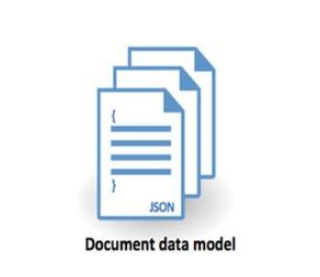
\includegraphics[scale=0.5]{images/nosql_documentos}
	\caption{Ejemplo de base de datos documental}
	\label{fig:nosql_documental}
\end{figure}

\subsubsection{Bases de datos orientadas a grafos}

Las bases de datos orientadas a grafos representan las entidades como nodos de un grafo y las relaciones como las aristas entre ellos. Utiliza una técnica llamada adyacencia libre de índice (index-free  adjacency) la cual consiste en que cada nodo tiene un puntero que apunta al nodo adyacente.  La  base  de  datos  debe  estar  totalmente  normalizada  para  poder  sacar  el  máximo rendimiento, es decir que cada tabla tendrá una sola columna y cada relación dos. De esta manera se puede adaptar el modelo de datos según las necesidades y poder recorrer millones de registros. Algunas bases de datos de este tipo son \textit{Neo4j, ArangoDB, AllegroGraph}.

\begin{figure}[!h]
	\centering
	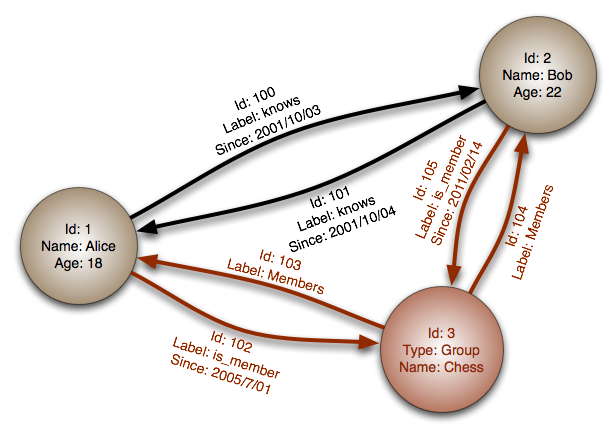
\includegraphics[scale=0.4]{images/nosql_grafos}
	\caption{Ejemplo de base de datos de grafos}
	\label{fig:nosql_grafos}
\end{figure}

\subsubsection{Bases de datos orientadas a columnas}

Son bases de datos similares a las bases de datos relacionales, aunque comparten el concepto de almacenamiento columna a columna de las bases de datos basadas en filas, los almacenes de columnas no almacenan los datos en tablas sino en arquitecturas distribuidas masivamente. En estos  almacenes  cada  clave  está  asociada  con  uno  o  más  atributos  (columnas).    Los  datos almacenados en la base de datos se basan en el orden determinado por la clasificación de la column family y se almacenan de manera contigua de tal forma que se realizan los accesos mucho más rápido. Algunas bases de datos de ese tipo son \textit{Cassandra, BigTable, HyperTable}.

\begin{figure}[!h]
	\centering
	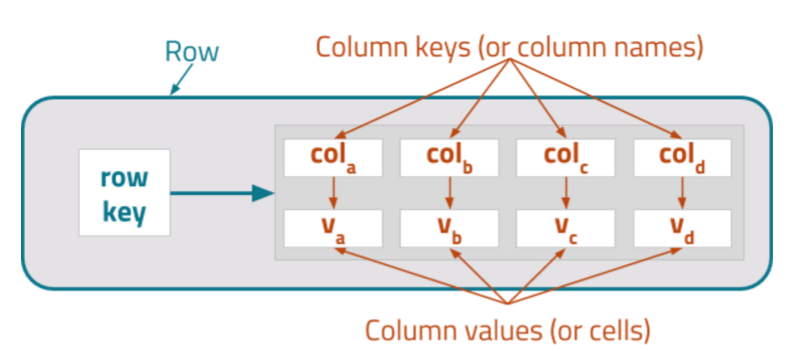
\includegraphics[scale=0.5]{images/nosql_columnas}
	\caption{Ejemplo de base de datos orientadas a columnas}
	\label{fig:nosql_columnas}
\end{figure}

\subsubsection{Bases de datos orientadas a objetos}

Son bases de datos en las cuales los datos o la información a almacenar se representan como un objeto (similar al de programación orientada a objetos). El almacén de datos ofrece todas las características  de  la  programación  orientada  a  objetos  tales  como  encapsulación  de  datos, polimorfismo y herencia. Las clases, los objetos y los atributos de clase son comparables a una tabla, una tupla y las columnas de la tupla. Cada objeto tiene un identificador que puede utilizarse para identificarlo de forma única. Las bases de datos orientadas a objetos deben utilizarse en aplicaciones que impliquen relaciones de objetos complejas o en las que cambien la estructura de objetos. Algunas bases de datos de este tipo son ObjectDB, db4o.

\begin{figure}[!h]
	\centering
	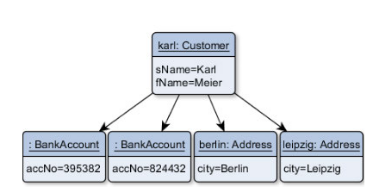
\includegraphics[scale=0.7]{images/nosql_objetos}
	\caption{Ejemplo de base de datos de objetos}
	\label{fig:nosql_objetos}
\end{figure}

\newpage

Las principales ventajas de este modelo son \cite{ref9}:

\begin{itemize}
	\item La \textbf{escalabilidad} y su carácter \textbf{descentralizado}. Soportan estructuras distribuidas.
	
	\item Suelen ser bases de datos mucho más \textbf{abiertas y flexibles}. Permiten adaptarse a necesidades de proyectos mucho más fácilmente que los modelos de Entidad Relación.
	    
	\item Se pueden hacer cambios de los esquemas sin tener que parar bases de datos.
	    
	\item \textbf{Escalabilidad horizontal}: son capaces de crecer en número de máquinas, en lugar de tener que residir en grandes máquinas.
	    
	\item Se pueden ejecutar en máquinas con pocos recursos.
	    
	\item Optimización de consultas en base de datos para grandes cantidades de datos.
\end{itemize}

Las principales inconvenientes de este modelo son \cite{ref9}:

\begin{itemize}
	\item No todas las bases de datos NoSQL contemplan la \textbf{atomicidad} de las instrucciones y la \textbf{integridad} de los datos. Soportan lo que se llama consistencia eventual.
	
	\item \textbf{Problemas de compatibilidad} entre instrucciones SQL. Las nuevas bases de datos utilizan sus propias características en el lenguaje de consulta y no son 100\% compatibles con el SQL de las bases de datos relacionales. El soporte a problemas con las queries de trabajo en una base de datos NoSQL es más complicado.
	
	\item \textbf{Falta de estandarización}. Hay muchas bases de datos NoSQL y aún no hay un estándar como sí lo hay en las bases de datos relacionales. Se presume un futuro incierto en estas bases de datos.
	
	\item \textbf{Soporte multiplataforma}. Aún quedan muchas mejoras en algunos sistemas para que soporten sistemas operativos que no sean Linux.
	
	\item Suelen tener \textbf{herramientas de administración no muy usables} o se accede por consola.
\end{itemize}

\newpage % Sección 5

\section{Comparativa SQL vs NoSQL}

\begin{wrapfigure}{L}{0.35\textwidth}
\vspace{-0.4cm}

\includegraphics[width=0.3\textwidth]{images/sql_o_nosql}
\end{wrapfigure}

Las bases de datos no son para nada ajenas a las innovaciones y nuevas tendencias que se desarrollan a su alrededor. Es por ello que a las tradicionales bases SQL les salió ya hace ya un tiempo un competidor que cada vez tiene más fuerza, las bases NoSQL. Muchos desarrolladores han optado por migrar sus proyectos y trabajos a este modelo, pero para hacerlo es conveniente primero saber las diferencias entre ambas y también sus principales tecnologías, de forma que puedas tener información precisa sobre cuál conviene más en cada caso.

\begin{figure}[H]
	\centering
	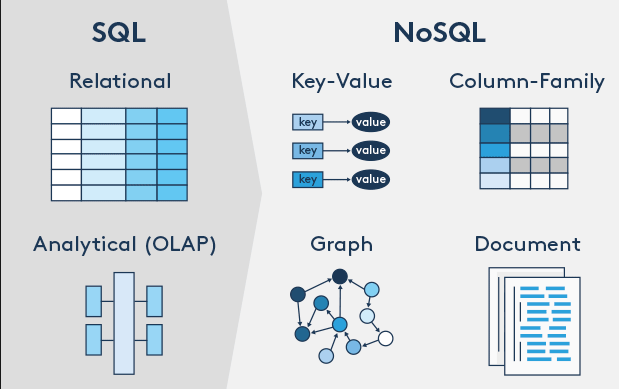
\includegraphics[scale=0.4]{images/comparativa_sql_vs_nosql}
	\caption{Comparativa SQL vs NoSQL}
\end{figure}

\subsection*{¿Cuándo utilizar qué tipo de base de datos?}

Entonces, ¿es NoSQL el sustituto directo para evolucionar de las antiguas bases de datos relacionales?. Esto no es cierto para todos los casos, sino que se tiene que tener en cuenta el diseño del problema para poder saber a qué modelo de base de datos se puede ajustar mejor.

A continuación se van a detallar las principales diferencias y contextos de uso.

\subsubsection*{Integridad de datos}

La integridad de datos es la garantía de que los datos almacenados mantendrán su exactitud y consistencia a través del tiempo. Tu código siempre deberá servir mientras tú mismo no modifiques su estructura.

\begin{itemize}

	\item \texttt{SQL:} Las tablas tienen estructuras rígidas, donde cada dato tiene un tipo definido, no podemos almacenar datos de otro tipo diferente, y no se vale más de un dato en un mismo campo. Puesto que todos los registros cumplen las mismas reglas, si tu código \textbf{funciona con un solo registro, servirá con todos los demás}.
	
	\item \texttt{NoSQL:} Hay varios tipos de base de datos NoSQL, pero en general, ninguna te exige que definas el tipo de datos que vas a almacenar. Un día un campo puede ser un número y al otro día un String o Array o hasta un JSON. Más que saber qué es la data, NoSQL pone mayor prioridad en cómo acceder dicha data.

\end{itemize}

\textsc{¿Qué significa esto?}

Que si necesitas que tus datos se mantengan \textbf{exactos y consistentes} a través del tiempo, \textbf{una base de datos SQL te lo garantiza}. Esto es lo ideal en muchos sistemas intolerantes a las fallas, donde mientras menos aberturas dejes, mejor (por ejemplo la mayoría, quizá totalidad, del software bancario y empresarial). Aquí SQL te cuida las espaldas.

Pero también, que si tus estructuras de datos son propensas a cambiar, el SQL te puede perjudicar al imponer una estructura rígida (por ejemplo, si estas en las fases de prototipo o lanzamiento temprano de una app, donde los datos que guardas son más maleables).

Mientras que \textbf{añadir llaves nuevas a un documento NoSQL suele ser muy fácil}, modificar tablas SQL puede traer muchos inconvenientes si ya el sistema funciona con cierta estructura, y más aún si hablamos de introducir cosas como llaves primarias.

\subsubsection*{Operaciones atómicas}

Una operación atómica es cuando haces un cambio que afecta a \textbf{múltiples entidades de la base de datos al mismo tiempo}. Esto suele acompañarse con el concepto de “transacciones”: decirle a la BD que, o cambian todas las tablas que queremos al mismo tiempo, o no cambia nada y la base de datos queda intacta (el famoso “rollback”, todo o nada).

\begin{itemize}

	\item \texttt{SQL:} Las bases de datos relacionales tienen atomicidad gracias a que sus tablas están conectadas y pueden “ponerse de acuerdo” para no aceptar cambios nuevos hasta que termine una transacción.
	
	Si tu sistema posee operaciones donde necesitas cambiar datos de varias entidades al mismo tiempo, ya es una alerta roja para usar SQL, pues estás reconociendo que hay relaciones entre los datos, y que éstas son importantes.
	
	Si además hablamos de \textbf{operaciones delicadas} (como procesar una factura, donde se suelen actualizar más cosas, por ejemplo el stock de un producto), es casi seguro que la atomicidad te salvará el pellejo de situaciones como que dos personas traten de pagar por el último de un producto al mismo tiempo.

	\item \texttt{NoSQL:} Datos no relacionales = no hay relaciones sobre las que hacer una transacción atómica. Simplemente, cuando quieres hacer cambios en 5 entidades diferentes, de frente o detrás de cámaras habrá 5 llamadas diferentes a la base de datos una detrás de otra.

\end{itemize}

\textsc{¿Qué significa esto?}

\texttt{NoSQL} no cuenta con \textbf{atomicidad}, y ésta \textbf{es vital para ciertos sistemas}.

¿La desventaja? \textbf{La atomicidad no es barata para la máquina}, consume capacidad de procesamiento y afecta el rendimiento de la base de datos, pues ésta hace el trabajo sucio para garantizar que nadie más se entrometa en una transacción.

¿Cuándo elegir \texttt{NoSQL}? \textbf{La atomicidad no siempre es crucial}.

Comparado con una inconsistencia en un estado de cuenta bancaria, ¿qué tan crítico es si dos usuarios difieren en la cantidad de likes de un post? \textbf{A veces la velocidad de respuesta es más importante} que la consistencia de datos (muchas app móviles caen en esto), y aquí brilla NoSQL.	

\subsubsection*{Escalabilidad}

Este suele ser un punto controversial cuando hablamos de cantidad de registros que podemos almacenar antes que la BD empiece a dar problemas. ¿La realidad? \textbf{Depende totalmente de la base de datos específica que usemos}.

Para empezar, cuando pensamos en escalabilidad es muy probable que realmente pensemos en \textbf{escalabilidad vertical}: aumentar el poder de una máquina para que pueda aguantar una mayor cantidad de datos.

Soluciones SQL como MySQL, Microsoft SQL Server y Postgre han probado su poder de escalar verticalmente a través de los años, pero NoSQL también tiene sus jugadores como Hadoop o Riak que, en sus respectivos campos (Big Data y soluciones distribuidas) aguantan datos como una montaña aguantando gotas de lluvia.

¿Entonces, donde hay mayor diferencia? En la \textbf{escalabilidad horizontal}, es decir, en cuántas máquinas diferentes podemos dividir la BD para repartir la carga.

\begin{itemize}

	\item \texttt{SQL:} La verdad es que la mayoría de soluciones SQL tienen buen soporte para escalar verticalmente.
	
	Pero cuando tratas de que la información en tu base de datos se mantenga consistente para todos los usuarios, los problemas llegan al hablar de miles y millones de registros. Aun con una máquina muy potente, puedes verte obligado a dividir tu base de datos entre diferentes procesadores y hasta servidores.
	
	Ahora, las bases de datos distribuidas SQL no son un concepto nuevo y compañías como Microsoft llevan años trabajando en ello, pero no es algo barato (para el bolsillo ni para el procesamiento).
	
	\textbf{Siempre hay cierto riesgo de presentar inconsistencias}, pues la BD ahora debe revisar que todo este en orden a través de diferentes máquinas.

	\item \texttt{NoSQL:} Cuando no tienes la consistencia de datos como prioridad, \textbf{distribuir y replicar} tu base de datos en múltiples máquinas \textbf{es trivial}, y por eso se considera que el NoSQL es excelente para bases de datos necesitan escalar horizontalmente (por ejemplo, en Big Data, donde una sola máquina se queda corta sumamente rápido).

\end{itemize}

\textsc{¿Qué significa esto?}

Las bases de datos relacionales ya vienen equipadas para crecer verticalmente, lo cual es más que suficiente para empresas pequeñas a grandes, proyectos personales, blogs y demás… hasta cierto punto, y mientras tengas \textbf{una buena máquina con la capacidad requerida}.

\texttt{NoSQL}, por el contrario, la tiene más fácil residiendo en \textbf{muchas máquinas menos potentes}.

\subsubsection*{Velocidad}

Esto es que tan rápidas son las lecturas y escrituras a la BD. Una necesidad básica, pero tan importante que \texttt{puede definir por sí sola con qué modelo nos quedamos}.

\begin{itemize}


\item \texttt{SQL:} Las garantías que te dan las relaciones conllevan un precio. Esto es más evidente cuando empezamos a hacer consultas con “joins” (que involucran múltiples entidades) y de repente una búsqueda \textbf{puede tardar minutos y hasta horas} debido a la gran cantidad de datos que está revisando.

Es un problema que se suele aliviar con buen diseño de la BD, pero está ahí y te morderá tarde o temprano.

\item \texttt{NoSQL:} Mientras que un buen diseño en SQL sirve para amortiguar un golpe, en NoSQL determinará que tanto jugo le saques a la velocidad con que viene.

Asumiendo que buscas tus datos de una sola entidad, las bases de datos no relacionales suelen contar con mecanismos de \textbf{búsqueda sumamente rápida} para conseguir un dato específico entre millones.

\end{itemize}

\textsc{¿Qué significa esto?}

Que si sabes cómo diseñar tu base de datos, es casi seguro que \textbf{una NoSQL bien diseñada gane por mucho en velocidad} a una SQL, haciéndolas sumamente atractivas para aplicaciones modernas donde los usuarios viven de su plan de datos, y donde si tu app no carga en un par de segundos ya piensan en desinstalar.

Siempre puedes optimizar ambos modelos hasta obtener un rendimiento aceptable, pero en NoSQL puedes \textbf{diseñar tu base de datos en función a las consultas que harás}, dándole una ventaja descomunal.


\subsubsection*{Consistencia vs redundancia}

Probablemente la diferencia más marcada entre ambos modelos, y donde más fácil nos es dejarnos llevar por nuestros conocimientos de SQL.

\begin{itemize}
\item \texttt{SQL:} La consistencia de datos es asegurarse de que un único dato este \textbf{una única vez en toda la base de datos}; y se suele lograr con el proceso de “Normalización” (reducir la cantidad de datos “repetidos” en la BD).

Esto garantiza que por ejemplo, si buscas el nombre de alguien, el nombre que verás es exactamente el mismo que podrían ver tu vecino o alguien en Pekín, si están conectados a la misma base de datos. Igual de importante, significa que mientras vayas navegando en tu app, si 10 pantallas diferentes cargan un dato, las 10 veces será el mismo dato.

\item \texttt{NoSQL:} La redundancia es repetir adrede los datos a conveniencia en varias partes de la BD (datos “de-normalizados”).

Por ejemplo, si almacenamos datos de una reservación hotelera, guardamos todos los datos de una persona en la entidad “Persona”. Pero además, guardamos una copia del nombre, teléfono y demás información personal en cada “Reservación” y posiblemente en cada “Factura” de esta persona.

Si cambian los datos de una persona en “Persona”, no necesariamente se reflejará este cambio en las otras entidades (ya esto queda a mano y decisión tuya); pero también hace que al buscar facturas o reservaciones, no tenemos que dar vueltas extra para obtener los datos de la persona.

\end{itemize}

\textsc{¿Qué significa esto?}

Algunas aplicaciones necesitan consistencia de datos, pero otras \textbf{prefieren el incremento en velocidad}. Recuerda que el espacio de almacenamiento es barato y solo se abarata más cada año, pero el procesamiento y los datos móviles aún son oro para los usuarios finales.

También, al diseñar bases de datos NoSQL, debes tener siempre en mente que \textbf{la redundancia está de tu lado}. Muchas veces nos quejamos al utilizar servicios como la Realtime Database de Firebase pues restringen nuestra capacidad para consultar diferentes colecciones (entidades) al mismo tiempo.

En realidad, están diseñados así para optimizar las consultas rápida, y el problema más común es que no aprovechamos al máximo la redundancia para poner la información que necesitamos en un único lugar.

\subsubsection*{Comodidad para el desarrollador}

\begin{itemize}


\item \texttt{SQL:} La comunidad SQL \textbf{lleva décadas madurando}, y esto se traduce no solo en mejores herramientas administrativas, sino en estándares mejores definidos, mayor documentación, y hasta comunidades más grandes de desarrolladores listos para ayudarte con tus problemas o unirse a tu equipo de trabajo.

\item \texttt{NoSQL:} Lo pondré así, buena suerte consiguiendo herramientas administrativas como phpMyAdmin y de manera gratuita. Aquí el punto fuerte es la conveniencia: factores como que los datos no necesiten tipos o que puedas aprovechar la redundancia, hacen \textbf{más flexible} el desarrollar con NoSQL.

Si estás prototipando, \textbf{los cambios son más rápidos y tienen menos consecuencias}. Si sabes qué quieres mostrar a tus usuarios, es fácil diseñar bases de datos especializadas en servir exacta y rápidamente la información que quieres.

\end{itemize}

\textsc{¿Qué significa esto?}

Que las base de datos \textbf{NoSQL te suelen dar más libertad para experimentar y equivocarte}, haciendo cambios a diestra y siniestra… pero éstas son necesidades que no tendrás siempre.

\textbf{Cuando tienes un sistema mejor definido}, te hará falta contar con buenas herramientas administrativas o saber que hay más gente ahí afuera lista para apoyarte o unirse a tu equipo rápidamente, y en esto \textbf{SQL brilla}.

En resumen, se puede decir que \textbf{NoSQL} te da más facilidades como desarrollador y \textbf{ventajas a corto plazo}, mientras que los beneficios de \textbf{SQL} los sueles ver cuando va pasando el tiempo y te toca \textbf{mantener el sistema}.

\vspace{1cm}

\begin{table}[H]
	\centering
	\begin{tabular}[c]{|l |l |l|}
		\hline
		\rowcolor{azulOscuro} \color{white}Característica & \color{white}NoSQL & \color{white}SQL \\
		\hline
		\cellcolor{azulClaro} Rendimiento & \cellcolor{verdeSuave}Alto & \cellcolor{rojoSuave}Bajo \\
		\cellcolor{azulClaro}Confiabilidad & \cellcolor{rojoSuave}Baja & \cellcolor{verdeSuave}Buena \\
		\cellcolor{azulClaro}Disponibilidad & \cellcolor{verdeSuave}Buena & \cellcolor{verdeSuave}Buena \\
		\cellcolor{azulClaro}Consistencia & \cellcolor{rojoSuave}Baja & \cellcolor{verdeSuave}Buena \\
		\cellcolor{azulClaro}Almacenamiento & \cellcolor{verdeSuave}Soporta enormes cantidades & \cellcolor{amarilloSuave}Cantidades medio/grande \\
		\cellcolor{azulClaro}Escalabilidad & \cellcolor{verdeSuave}Alta & \cellcolor{amarilloSuave}Alta pero más cara \\
		\hline
	
	\end{tabular}
	\caption{Resumen de las características NoSQL y SQL}
\end{table}


\newpage % Sección 6

\section{Conclusiones}

Muchas personas piensan que las tecnologías NoSQL son lo “nuevo” y por lo tanto todo debe migrar a este modelo, pero es un grave error. NoSQL no es un reemplazo, es simplemente un modelo diferente que ofrece ventajas y soluciones a problemas que poseen las bases de datos relacionales \cite{ref8}.

Si tu proyecto necesita una \textbf{escalabilidad importante}, donde los recursos son escasos (hardware, procesamiento, etc.) y \textbf{no necesita respetar la integridad de los datos}, por ejemplo, una aplicación para IOT con millones de dispositivos reportando valores de sensores, redes sociales o \textbf{desarrollos de Big Data} que presentan retos a las bases de datos tradicionales, entonces sí: \texttt{NoSQL} es la mejor opción.

Si el proyecto necesita que se \textbf{respete la integridad de los datos}, por ejemplo, una aplicación para un banco, inteligencia y análisis de negocios para la identificación de patrones en los datos, software a medida o software empresarial que necesitan información con estructura \textbf{consistente} o desarrollos web donde la \textbf{jerarquía de datos} es importante, \texttt{SQL} será la mejor opción.


\newpage % Sección 7


\begin{thebibliography}{99}

\bibitem{ref1} José Miguel Rojas Gonzales, Análisis comparativo de bases de datos relacionales y no relacionales, disponible en: \url{http://oa.upm.es/48941/1/TFG_JOSE_MIGUEL_ROJAS_GONZALES.pdf}

\bibitem{ref2} Rafael Camps Paré, Luis Alberto Casillas Santillán, Dolors Costal Costa, Marc Gibert Ginestà, Carme Martín Escofet, Oscar Pérez Mora, Bases de datos, página 5, disponible en \url{https://www.uoc.edu/masters/oficiales/img/913.pdf}

\bibitem{ref3} Victor Olaya, Sistemas de información geográfica, Parte2, bases de datos, disponible en:  \url{http://volaya.github.io/libro-sig/chapters/Bases_datos.html}

\bibitem{ref4} Tecnologias-informacion.com, Bases de Datos: Tipos y Usos, disponible en:  \url{https://www.tecnologias-informacion.com/basesdedatos.html}

\bibitem{ref5} Sistemas de gestión de bases de datos, sección 1.5, disponible en: \url{https://gestionbasesdatos.readthedocs.io/es/latest/Tema1/Teoria.html}

\bibitem{ref6} Joselín Rivero, Bases de datos en la actualidad, disponible en: \url{https://es.scribd.com/document/271755314/La-Base-de-Datos-en-La-Actualidad}

\bibitem{ref7} campusmvp.es, Diseñando una base de datos en el modelo relacional, disponible en:  \url{https://www.campusmvp.es/recursos/post/Disenando-una-base-de-datos-en-el-modelo-relacional.aspx}

\bibitem{ref8} Slashmobility, NoSQL vs SQL: ¿cuál elegir?, disponible en: \url{https://slashmobility.com/blog/2016/12/nosql-vs-sql-cual-elegir/}

\bibitem{ref9} Pandorafms, NoSQL vs SQL: principales diferencias y cuándo elegir cada una de ellas, disponible en: \url{https://blog.pandorafms.org/es/nosql-vs-sql-diferencias-y-cuando-elegir-cada-una/}

\end{thebibliography}

\end{document}